\begin{figure}[H]
\centering
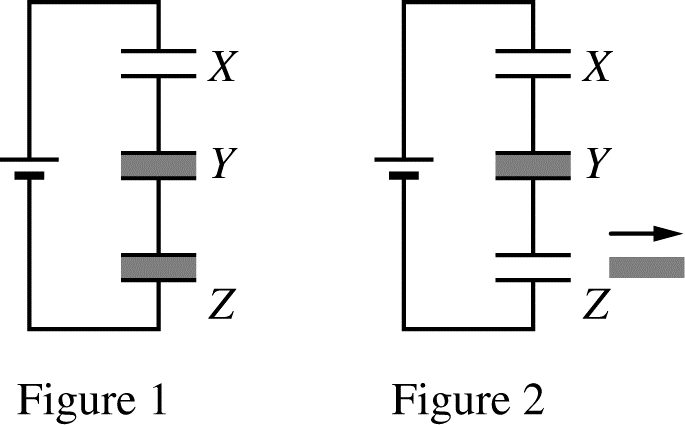
\includegraphics[scale=0.3]{images/img-006-010.png}
\end{figure}

% Multiple Choice Question 10
\begin{questions}\setcounter{question}{9}\question
Three capacitors are connected in series to an ideal voltage source and charged, as shown in Figure 1 above. The capacitors are identical except that capacitor $X$ has air between its plates, whereas capacitors $Y$ and $Z$ each have a dielectric slab of dielectric constant $\boldsymbol{\kappa}>1$ between their plates. If the dielectric slab is removed from capacitor $Z$, as shown in Figure 2, which of the following describes what will happen to the voltage across each capacitor?

\tabto{0.75cm} Voltage across
\tabto{4.00cm} Voltage across
\tabto{7.25cm} Voltage across\\
\tabto{0.75cm} \underline{Capacitor $X$}
\tabto{4.00cm} \underline{Capacitor $Y$}
\tabto{7.25cm} \underline{Capacitor $Z$}

\begin{choices}
\choice Increases \tabto{3.25cm} Increases \tabto{6.50cm} Decreases
\choice Increases \tabto{3.25cm} Decreases \tabto{6.50cm} Decreases
\choice Increases \tabto{3.25cm} Decreases \tabto{6.50cm} Increases
\choice Decreases \tabto{3.25cm} Increases \tabto{6.50cm} Decreases
\choice Decreases \tabto{3.25cm} Decreases \tabto{6.50cm} Increases
\end{choices}\end{questions}
